%% CDC 2019
% *****************************************************

\blfootnote{The content of this chapter is an adaptation of the following three papers:
\begin{enumerate}
    \item \bibentry{de2020access}.
    \item \bibentry{de2020approximation}.
    \item \bibentry{mohamed2019imacs}.
\end{enumerate}
}
\Gls{ibc} systems are common in many modern applications. 
In such systems, image-based sensing imposes massive compute workload, making it challenging to implement them on embedded platforms. 
Approximate image processing is a way to handle this challenge. In essence, approximation reduces the workload at the cost of additional sensor noise. In this work, we propose an approximation-aware design approach for optimizing the memory and performance of an \gls{ibc} system, making it suitable for embedded implementation. We perform compute- and data-centric approximations and evaluate their impact on the memory utilization and closed-loop \gls{qoc} of the \gls{ibc} system. Further, an \gls{ibc} system operates under several environmental scenarios, e.g., weather conditions. We evaluate the sensitivity of the \gls{ibc} system to our approximation-aware design approach when operated under different scenarios and perform a \gls{fp} analysis using Monte-Carlo simulations to analyze the robustness of the approximate system. Further, we design an optimal approximation-aware controller that models the approximation error as sensor noise and show \gls{qoc} improvements. In essence, this is an alternative design paradigm in the \gls{spade} flow to deal with high compute workload, complementary to parallelisation and pipelining. We demonstrate the effectiveness of our approach through the \gls{lkas} case study using  a  heterogeneous  NVIDIA AGX  Xavier  embedded platform  in  a  \gls{hil} framework. Both the platform and the \gls{lkas} case study were already introduced in Chapter \ref{chap:intro}.
We show substantial memory reductions and \gls{qoc} improvements with respect to the accurate implementation.
Approximate computing also helps to improve energy efficiency of our design. This last aspect of the work, reported in~\cite{de2020access}, is excluded in this thesis as it is not the primary focus of this thesis.

\section{Background and contributions}
\begin{figure}[tb]
\vspace*{-1.5ex}
    \centerline{
     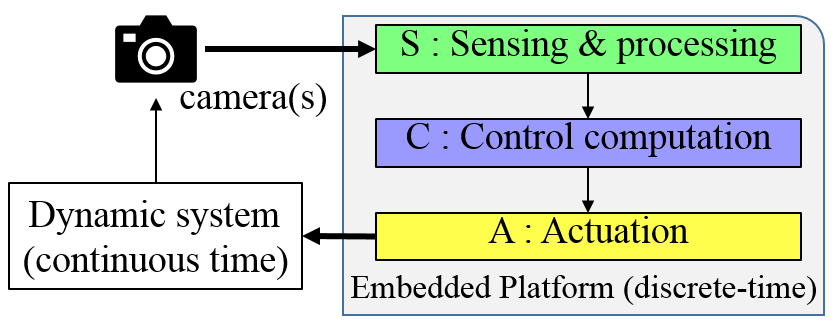
\includegraphics[width=0.6\textwidth]{images/IBC_bd2.png}
    }
    \vspace*{-1.5ex}
    \caption{An \gls{ibc} system: block diagram (repeating Fig.~\ref{fig:ch1_ibc_intro}~(a), for readability)}
    \label{fig:ch3_IBC_block_diagram}
    %\vspace{-2em}
\end{figure}

\Gls{ibc} systems are a class of data-intensive feedback control systems having camera(s) as the sensor (see Fig.~\ref{fig:ch3_IBC_block_diagram}). \Gls{ibc} has become popular with the advent of efficient image-processing systems and low-cost \gls{cmos} cameras with high resolution~\cite{corke2017robotics}\cite{van2018data}. The combination of the camera and image processing (sensing) gives necessary information on parameters such as relative position, geometry, relative distance, depth perception and tracking of the object-of-interest. This enables the effective use of low-cost camera sensors to enable new functionality or replace expensive sensors in cost-sensitive industries like automotive~\cite{corke2017robotics}\cite{pendleton2017perception}\cite{saidi2018future}.

A typical implementation of an \gls{ibc} system uses \gls{lqr} control~\cite{dorf2011modern} and considers the worst-case workload~\cite{saidi2018future}.
However, this leads to a long sensing delay, poor effective resource utilisation in the multiprocessor platform, and suboptimal \gls{qoc}~\cite{saidi2018future}. 
Fig.~\ref{fig:ch3_workload_IBC} illustrates these challenges.
The camera captures an image stream at a fixed frame rate (\gls{fps}). 
The execution times of the compute-intensive processing (sensing) of the image stream depend on image workload variations. The workload variations occur due to image content and result in a wide range between best-case and the worst-case image-processing times. 

\begin{figure}[tb]
\centerline{
    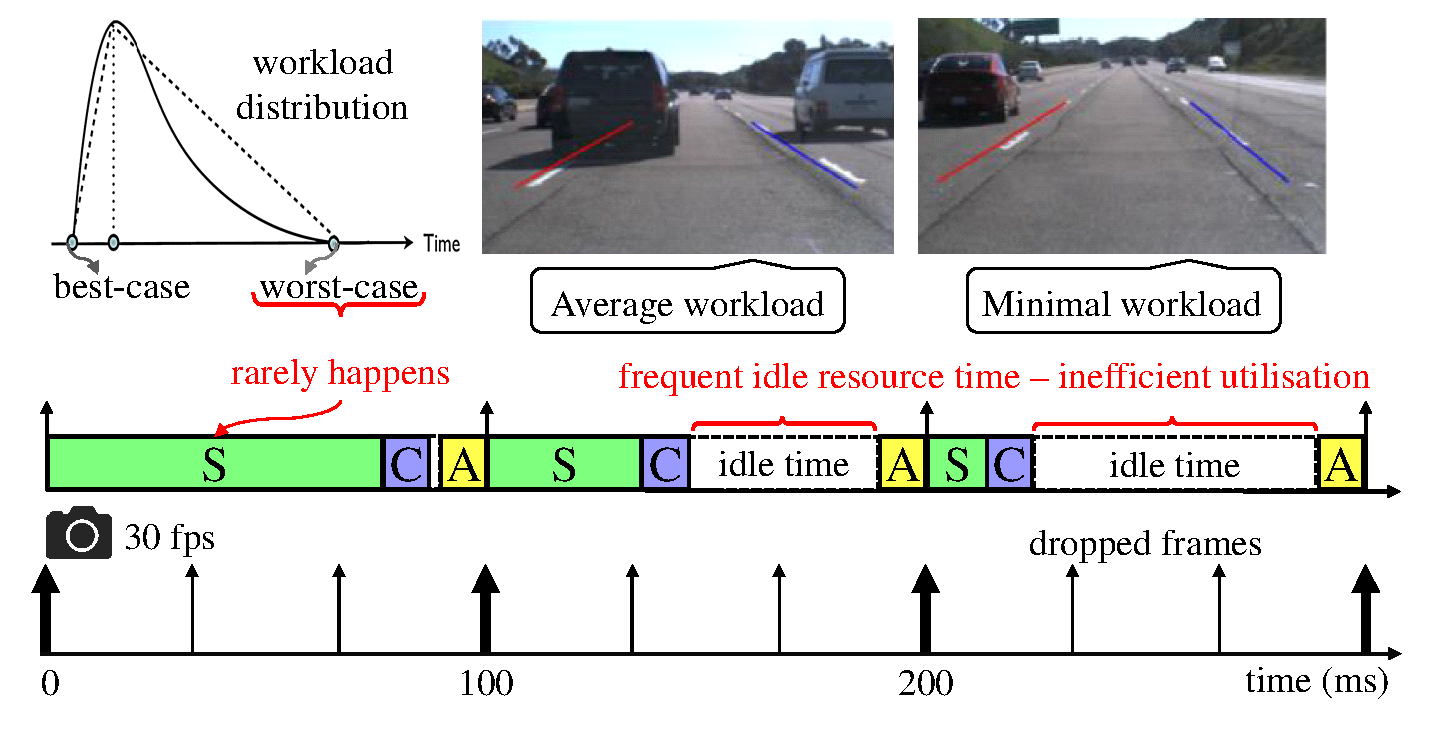
\includegraphics[width=\textwidth]{images/workload_IBC.eps}
    }
    \caption{Illustration of \gls{ibc} system implementation and challenges for \gls{lqr} control design considering worst-case workload. \taskS: sensing and image processing, \taskC: control computation and \taskA: actuation, see Fig.~\ref{fig:ch3_IBC_block_diagram}. (Adapted from Fig.~\ref{fig:ch5_intro}, for readability.)}
    \label{fig:ch3_workload_IBC}
    \vspace{-2em}
\end{figure}

The workload variations can, however, be statistically analysed, e.g., as a PERT distribution~\cite{adyanthaya2014robustness} or \gls{dtmc}~\cite{welton2005estimation}, from observed data and can be modelled as workload scenarios (explained in Chapter~\ref{chap:parallelisation}).
 The workload scenarios can be modelled (e.g. as a task graph or a dataflow graph), analysed (for timing) and then mapped to a multiprocessor platform. 
 A system scenario abstracts multiple workload scenarios having the same sampling period as determined by platform constraints.
 An optimal mapping and controller may then be designed for each system scenario. 
 
For efficiently designing \gls{ibc} systems, we should consider the workload variations and the given platform allocation. 
An ideal design approach should: (i) identify, model and characterise the workload scenarios; (ii) find optimal mappings for these workload scenarios for the given platform allocation; (iii) identify optimal system scenarios; and (iv) design a controller with high overall \gls{qoc} for the chosen system scenarios.
One of the critical aspects here is: what is a good metric to define the \gls{qoc} for the application? 
A vision-guided braking application requires a fast settling time, whereas an automotive vision-based lateral control~\cite{taylor1999comparative} application requires to minimise the reference tracking error.

 Section \ref{chap:spadeoverview} introduces the \gls{spade} approach for designing \gls{ibc} systems.  \gls{spade} characterises a set of frequently occurring workload scenarios, identifies a set of system scenarios that abstract multiple workload scenarios based on platform constraints, and designs a switched linear control system for these system scenarios to improve \gls{qoc}.   
 However, if the number of switching subsystems is high, a challenge in \gls{spade} is the difficulty to guarantee stability for the resulting switched system~\cite{mohamed2018optimising, van2018data}.
In case of failure to guarantee stability, \gls{spade} as developed so far in the earlier chapters would result in \gls{lqr} control for the worst-case workload scenario.

The contributions of this chapter are as follows:
 \begin{itemize}
     \item We present an alternate controller synthesis method based on a \gls{mjls} formulation for the control design step in the full \gls{spade} approach of Chapter~\ref{chap:pipelined_parallelism}. Our synthesis method involves the following steps. (i) Modelling workload variations as a \gls{dtmc}, (ii) system scenario identification, and (iii) controller design and implementation. The motivation to choose the \gls{mjls} approach~\cite{costa2006discrete} over other standard sampled-data linear control design techniques~\cite{ogata1995discrete} is that it does not require us to know the exact sequence of incoming sample times due to the workload variations apriori.
     \item We provide design guidelines on the applicability of control design methods for given requirements, implementation constraints and system knowledge. For this, we compare the three control paradigms -- optimal control design using \gls{lqr}, switched linear control design~\cite{van2018data}, and controller synthesis using the \gls{mjls} formulation
     -- for \gls{ibc} system design with respect to \gls{qoc} while taking into account available system knowledge and implementation constraints, i.e., camera fps, platform allocation and mapping. 
     Note that we cannot compare with adaptive~\cite{goodwin1980discrete} or model predictive control~\cite{bemporad2002model} approaches since we do not know the exact sequence of occurrence of incoming sample times due to the workload variations apriori.
 \end{itemize}

\section{Embedded image-based control}~\label{sec:ch3_ProblemSetting}
We consider a setting for an \gls{ibc} system as shown in Fig.~\ref{fig:ch3_IBC_block_diagram}. Our sensor is the camera module that captures the image stream.
The image stream is then fed to an embedded platform, e.g., a \gls{mpsoc}, at a fixed frame rate (fps), e.g., 30 fps. The tasks in our \gls{ibc} application - compute-intensive image sensing and processing (\taskS), control computation (\taskC) and actuation (\taskA) -
are then mapped to run on this \gls{mpsoc}.

\subsection{\Gls{lti} systems}~\label{sec:ch3_LTI}
We consider an \gls{lti} system of the following form:
\begin{align}
\dot{x}(t) &= \Acont x(t) + \Bcont u(t), \label{eq:ch3_contsys}\\
y(t) &=  \Ccont x(t),\nonumber
\end{align}
where $x(t) \in \Real^n$ represents the {\it state}, $y(t) \in \Real$ represents the {\it output}  and $u(t) \in \Real$ represents the control {\it input} of the system at any time $t \in \Real_{\geq 0}$. $\Acont$, $\Bcont$ and $\Ccont$ represent the state, input and output matrices of the system, respectively. 

We illustrate our work using the motivating case study of a vision-based lateral control system model explained in Section \ref{sec:lkas_case_Study}. We consider the \gls{lti} model with $v_x=15$$m/s$, and
\\

%\vspace{2em}
\scalebox{0.8}{
  $\Acont = \left[
  \begin{array}{rrrrr}
    -10.06 & -12.99 & 0 & 0 & 0\\
    1.096 & -11.27 & 0 & 0 & 0\\
    -1.000 & -15.00 & 0 & 15 & 0\\
    0 & -1.000 & 0 & 0 & 15\\
    0 & 0 & 0 & 0 & 0\\
  \end{array}
\right],\ \Bcont=\left[
  \begin{array}{c}
    75.47\\
    50.14\\
    0\\
    0\\
    0\\
  \end{array}
\right].$ \\
}
\\[1.5ex]
The fifth system state captures the curvature of the road at the look-ahead distance. The fifth state is required for observability of road curvature. The control input $u(t)$ is the front wheel steering angle $\delta_f$ and the output $y(t)$ is the look-ahead distance $y_L$ leading to $\Ccont = [0\ 0\ 1\ 0\ 0]$.

\subsection{Implementation, control law and control configurations}~\label{sec:ch3_control law}
The discrete-time control implementation we consider is already explained in Section~\ref{sec:ch5_embedded_implementation}.
The control input $u[k]$ is a \emph{state feedback} controller of the following form,
 \begin{align}
		u[k] = \Kgain_{\workloadScenario} z[k] + \Fgain_{\workloadScenario} \controlRef \nonumber
% 		\label{eqn:u}
 \end{align}
where $\Kgain_{\workloadScenario}$ is the state feedback gain and $\Fgain_{\workloadScenario}$ is the feedforward gain both designed for the workload scenario $\workloadScenario$. $\controlRef$ is the reference value for the controller. The approaches we use for designing the gains are explained in Section~\ref{sec:ch3_control_design}.

For each workload scenario $\workloadScenario$, we then define a control configuration $\Configuration_{\workloadScenario}^c$ as a tuple $\Configuration_{\workloadScenario}^c = (h_{\workloadScenario},\tau_{\workloadScenario}, \Kgain_{\workloadScenario}, \Fgain_{\workloadScenario})$.
\section{\texorpdfstring{\Gls{ibc}}{IBC} model, mapping and configurations}~\label{sec:ch3_sys_model}
In this chapter, we consider the \gls{sadf} model of Fig. \ref{fig:ch5_SADF}(a) with the same execution time parameters as our application model. The modelling, mapping and analysis of this \gls{sadf} model has already been explained in detail in Chapter \ref{chap:parallelisation} and is not repeated here. 
In Chapter \ref{chap:parallelisation}, the workload variations are characterised using a PERT distribution~\cite{adyanthaya2014robustness} (see distribution in Fig.~\ref{fig:ch3_workload_IBC}). Using this information, the probability of frequently occurring workload scenarios are characterised. However, information regarding scenario transitions is not captured. This means that any arbitrary order for scenario switching sequences needs to be considered in the language of the \gls{sadf} model.

In the \gls{mjls}-based approach, the workload variations are characterised using a \gls{dtmc} that takes into account the scenario transition probabilities. The states of the \gls{dtmc} model the workload scenarios (see Section~\ref{sec:ch3_MJLS}) and the transitions in the \gls{dtmc} model the scenario transitions. This means that the \gls{dtmc} determines the language of the \gls{sadf} model~\cite{theelen2006scenario}.
\section{Control problem and \texorpdfstring{\gls{qoc}}{QoC} metrics}~\label{sec:ch3_control_problem}
We consider a regulation problem for the \gls{ibc} system. That is, the control objective is to design $u[k]$ such that $y[k] \rightarrow \controlRef$ (a constant reference) as $k \rightarrow \infty$. 
The control objectives can be performance-oriented, control effort/energy-oriented or a combination of both. The control performance quantifies, in essence, how fast the output $y[k]$ reaches the reference $\controlRef$.  The control effort is the amount of energy or power necessary for the controller to perform regulation. 
The control performance and effort are parameters that can be tuned in the cost function for the \gls{lqr} design and \gls{mjls} synthesis using the state and input weights. We evaluate \gls{qoc} of an \gls{ibc} application considering the following metrics: two commonly used control performance metrics - \gls{mse} (explained in Section \ref{sec:ch5_MSE}) and \gls{st} (explained in Section \ref{sec:ch7_QoC_metrics}) and two commonly used metrics to evaluate control effort/energy - \gls{psd} and \gls{mce}. 
 
\noindent\textbf{\Acrfull{psd}:}
The \gls{psd} of a signal describes the power present in the signal as a function of frequency, per unit frequency. It tells us where the average power is distributed as a function of frequency.
We use Welch's overlapped segment averaging spectral estimation method~\cite{welch1967use} to compute \gls{psd} of our control input.
Lower \gls{psd} for the control input signal implies that the energy required is less and hence \gls{qoc} is better.

\noindent\textbf{\Acrfull{mce}:}
We define the maximum control effort as $\max_{k} \norm{u[k]}$.
A lower \gls{mce} means better \gls{qoc}. \gls{mce} can also be used to identify input saturation, if any.
\section{Control design}~\label{sec:ch3_control_design}
The control design technique we choose decides the controller feedback and feedforward gains $\Kgain$ and $\Fgain$ for the control law defined in Section~\ref{sec:ch3_control law}. To design a controller, we assume that the sampling period $h_i$ and sensor-to-actuator delay $\tau_i$ are known.
\subsection{\Gls{mjls} synthesis}~\label{sec:ch3_MJLS}
In this section, we characterise the workload variations as a \gls{dtmc}. The states of a \gls{dtmc} model the workload scenarios and the transitions model the scenario switching. We aggregate workload scenarios into system scenarios as explained in Section~\ref{sec:ch5_ch5_sys_scenario}, and then recompute transition and steady-state probabilities for the \gls{dtmc}. This results in a \gls{dtmc} with number of states equal to the number of identified system scenarios, with each state representing a system scenario. 
We assume that the switching between the different control configurations is governed by this \gls{dtmc} and show how the system in \eqref{eq:ch3_contsys} can be re-cast as a \gls{mjls}~\cite{costa2006discrete}. For the sake of simplicity, we illustrate the formulation using only three states in the \gls{dtmc} representing three system scenarios. Note, however, that it is applicable to any number of identified system scenarios (as explained in Section~\ref{sec:ch5_ch5_sys_scenario}).

A Markov chain consists of a tuple $\mathcal{M} = (X, P)$ where $X$ represents the state space, and $P$ represents the one-step transition probability matrix. In our context of system scenarios annotated with sampling period and sensor-to-actuator delay, the state-space of $\mathcal{M}$ is given by $X = \{s_1, s_2, s_3\}$, 
where $s_i = (h_i,\tau_i), i \in \{1,2,3\}$ represent three system scenarios, and \begin{align}
P = 
\begin{bmatrix}
p_{11} & p_{12} & p_{13} \\
p_{21} & p_{22} & p_{23} \\
p_{31} & p_{32} & p_{33} \nonumber
\end{bmatrix}.
\end{align}
Associated with $\mathcal{M}$ is a discrete-time stochastic process $\theta : \Natural \rightarrow X$ such that for all times sampling instances $k \in \Natural$, and states $s_i, s_j \in X$, $i,j \in \{1,2,3\}$, one has:
\begin{align}
\mathsf{Prob}(\theta[k+1] = s_j \mid \theta[k] = s_i) = p_{ij}, \nonumber 
\end{align}
i.e., $p_{ij}$ represents the probability of transitioning from state $s_i$ to $s_j$. We assume that the initial condition of the stochastic process, i.e., $\theta[0]$, is deterministic. 

Using a zero order sample-and-hold approach, it can be readily shown that Eq.~\eqref{eq:ch3_contsys} can be re-formulated into an \gls{mjls} governed by the following stochastic difference equations:
\begin{align}
x[k+1] &= A_{\theta[k]}x[k] + B_{0,\theta[k]}u[k] + B_{1,\theta[k]}u[k-1], \nonumber\\
y[k] &= \Ccont x[k]
~\label{eq:mjls}
\end{align}
where for each $s_i \in X$, $i \in \{1,2,3\}$: $A_{s_i},\ B_{0,s_i},$ and $B_{1,s_i}$ are computed using Eq.~\ref{eq:ch5_ch5_A_sk}.
In Eq.~\ref{eq:mjls}, we assume that $u[-1] = 0$ for $k = 0$. We define the new system states $z[k] = \begin{bmatrix}x[k] & u[k-1]\end{bmatrix}^T$ with $z[0] = \begin{bmatrix}x[0] & 0\end{bmatrix}^T$ to obtain a higher-order augmented system as follows:
\begin{align}
z[k+1] &= A_{aug,\theta[k]}z[k] + B_{aug,\theta[k]}u[k],\nonumber \\
y_z[k] &= C_{aug}z[k] \nonumber
\end{align}
where for each $s_i \in X, i \in \{1,2,3\}$, $A_{aug,s_i}$  and  $B_{aug,s_i}$ are computed using Eq.~\ref{eq:ch5_ch5_aug} and $C_{aug}=
\begin{bmatrix}
\Ccont & 0
\end{bmatrix}$. 
\\

\noindent\textbf{Infinite-horizon quadratic optimal controller:}
Here, we present the control law design for the \gls{mjls} of Eq.~\ref{eq:mjls}. We design a controller to minimize the infinite-horizon cost given by

\begin{equation}
J(\theta[0], z[0], u[0]) = \sum\limits_{k=0}^{\infty} \mathds{E}[z[k]^TC_{aug}^TC_{aug}z[k] + d_u^2|u[k]|^2],\nonumber
\end{equation}
where $d_u \in \Real_{>0}$ represents the input weight and the notation $\Expectation{X}$ represents the expected value of a random variable $X$. 

It is shown in \cite{costa2006discrete} that the solution to the above infinite-horizon optimal-control problem can be obtained by solving the {\it coupled algebraic Riccati (matrix) equations} (CARE) 
\small
\begin{align}
\label{eq:care}
&\Gamma_{i} = \Aaugi^T\mathcal{E}_{i}(\Gamma)\Aaugi + \Ccont^T\Ccont \nonumber\\
&- \Aaugi^T\mathcal{E}_i(\Gamma)\Baugi (\Baugi^T\mathcal{E}_i\Baugi)^{-1}\Baugi^T\mathcal{E}_i(\Gamma)\Aaugi \nonumber
\end{align}
\normalsize
 %\vspace{-2em}
 where
 \vspace{-2em}
\begin{align}
\mathcal{E}_i(\Gamma) = \sum\limits_{j = 0}^{3} p_{ij}\Gamma_j \nonumber
\end{align}
where $i \in\{1,2,3\}$ and $\Gamma = \{\Gamma_1,\Gamma_2, \Gamma_3\}$ are the unknown matrices to be solved for. The mean-square stabilizing optimal control law is then given by
\begin{align}
u[k] = \Kgain_{\theta[k]}(\Gamma) x[k] + \Fgain_{\theta[k]} \controlRef, \nonumber
\end{align}
where 
\begin{align}
\Kgain_{\workloadScenario} &= -(\Baugi^T\mathcal{E}_i(\Gamma)\Baugi)^{-1}\Baugi^T\mathcal{E}_i(\Gamma)\Aaugi,\nonumber \\
\Fgain_{\workloadScenario} &= \frac{1}{C_{aug}(I - \Aaugi - \Kgain_{\workloadScenario}\Baugi))^{-1} \Baugi},\nonumber
\end{align}
where $i \in\{1,2,3\}$. It is shown in Theorem A.12 in \cite{costa2006discrete} that the above CARE can be solved by solving a related convex optimization problem.

In the context of \gls{spade}, the control configuration for a workload scenario $\workloadScenario$ is then ($\tau_{\workloadScenario},\ h_{\workloadScenario},\ \Kgain_{\workloadScenario},\ \Fgain_{\workloadScenario}$).
\subsection{\Gls{lqr} design with worst-case workload}~\label{sec:ch3_LQR}
We consider the system scenario for the worst-case workload $s_{wc}$ having the worst-case period and delay $(h_{wc},\tau_{wc})$ (one of the scenarios as explained in Section~\ref{sec:ch5_ch5_sys_scenario}) for designing the control law. The worst-case system scenario for the \gls{mjls} formulation is same as $s_{wc}$. We design a controller to minimize the following cost function
\begin{align}
J(u) = \sum\limits_{k=0}^{\infty} z[k]^Td_sC_{aug}^TC_{aug}z[k] + d_u^2|u[k]|^2,\nonumber
\end{align}
where $d_u,d_s \in \Real_{>0}$ represents the input weight and the state weights respectively. The weights are optimized for the considered \gls{qoc} metric. Typically, $d_u\ll d_s$ so as to optimise for control performance and $d_u\gg d_s$ to optimise for control energy (see Section~\ref{sec:ch3_observations}).
\subsection{Switched linear control design}~\label{sec:ch3_SPADe}
The switched linear control design we consider is explained in Section \ref{sec:ch5_embeddedIBC}. This is the basic principle used in the controller designs presented in Chapters \ref{chap:parallelisation} and \ref{chap:pipelined_parallelism}. Frequently occurring workload scenarios are characterised using the the PERT distribution. A set of optimal system scenarios are identified. \gls{lqr} controllers are designed for each of these scenarios $s_s$ with $(h_s,\tau_s)$ that minimises the cost function given in Section~\ref{sec:ch3_LQR}. Further, the stability of this switched system is analysed by deriving \glspl{lmi} that check for the existence of a \gls{cqlf}.

\section{Results, observations and guidelines}~\label{sec:ch3_Results}
We consider the case-study of vision-based lateral
control for a vehicle (explained in Section~\ref{sec:ch3_ProblemSetting}) for comparison of the three approaches
for control design with respect to the \gls{qoc} metrics described
earlier. The controllers for \gls{lqr} and switched linear control are tuned for the corresponding \gls{qoc} metric evaluation by adjusting the input and state weights. 

\subsection{Simulation results}
We illustrate an instance of our simulation that compares the three control paradigms: (i) for a reference output profile (for the control state $y_L$) shown in Fig.~\ref{fig:ch3_results} (a), we see that the \gls{slc} settles faster than both the \gls{mjls} and \gls{lqr} designs; and (ii) for control input shown in Fig.~\ref{fig:ch3_results} (b), we see that minimum control effort is needed for \gls{lqr}. \gls{slc} needs the highest control effort and might violate the input saturation requirements, if any. The control metrics \gls{psd} and \gls{mce} are derived from the control input $u[k]$ plots (e.g., see Fig.~\ref{fig:ch3_results}~(b)) and focus on minimizing the control effort or energy, whereas the control metrics \gls{mse} and \gls{st} are derived from the considered control output $y_L$ plots (e.g., see Fig.~\ref{fig:ch3_results}~(a)) and focus on improving the performance of the system output.  

We consider for the above simulation instance a frame rate of 30 fps, i.e., $\fh=\frac{1}{30}=33.33\ ms$ and an allocation of two processors. Then, we characterise the workload variations of a synthetic data set using a \gls{dtmc} model.
We notice that the $(h_i,\tau_i)$ for the worst-case workload $s_{wc}$ for this allocation is $(100,74)\ ms$. We then identify (as explained in Section \ref{sec:ch5_ch5_sys_scenario}) the three possible system scenarios $\{s_1=(\fh,33),\ s_2=(2\fh,57),\ s_3=s_{wc}=(3\fh,74)\}\ ms$. The transition probability matrix of the \gls{dtmc} model considered in this case for the three scenarios is: 
\begin{align}
P = 
\begin{bmatrix}
0.5 & 0.25 & 0.25 \\
0.25 & 0.5 & 0.25 \\
0.25 & 0.25 & 0.5 \nonumber
\end{bmatrix}.
\end{align}
The three controllers are then designed for the above scenarios as explained in Section~\ref{sec:ch3_control_design} using the input weight $d_u=1$. 

The control performance is then evaluated for the \gls{qoc} metrics (defined in Section~\ref{sec:ch3_control_problem}) - \gls{mse}, \gls{st}, \gls{psd}, \gls{mce} and combinations of \gls{mse}/\gls{st} with \gls{psd}/\gls{mce}. The combinations of \gls{mse}/\gls{st} with \gls{psd}/\gls{mce} is considered as they are contradictory in nature and optimising both together is a challenge and often times necessary.
% \scalebox{0.8}{
\begin{figure*}[t!]
    \centering
    \begin{subfigure}[t]{0.5\textwidth}
        \centering
        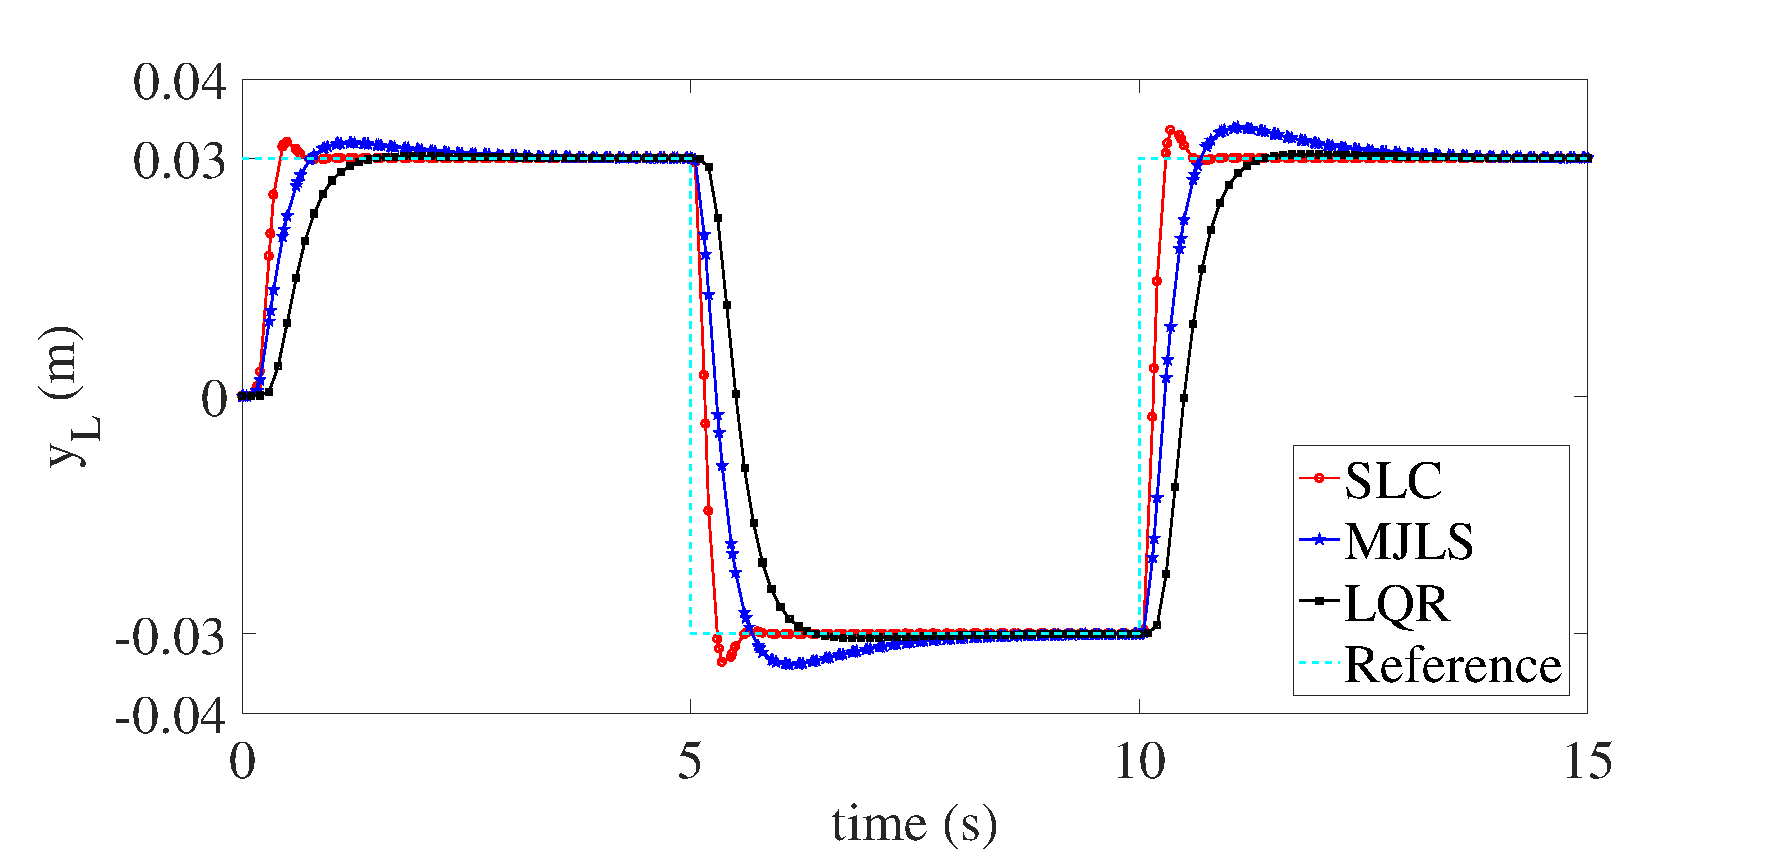
\includegraphics[width=\textwidth]{images/res_yL_R1.eps}
        \caption{Output $y_L$ when input weight $d_u=1$.}
    \end{subfigure}%
    ~ 
    \begin{subfigure}[t]{0.5\textwidth}
        \centering
       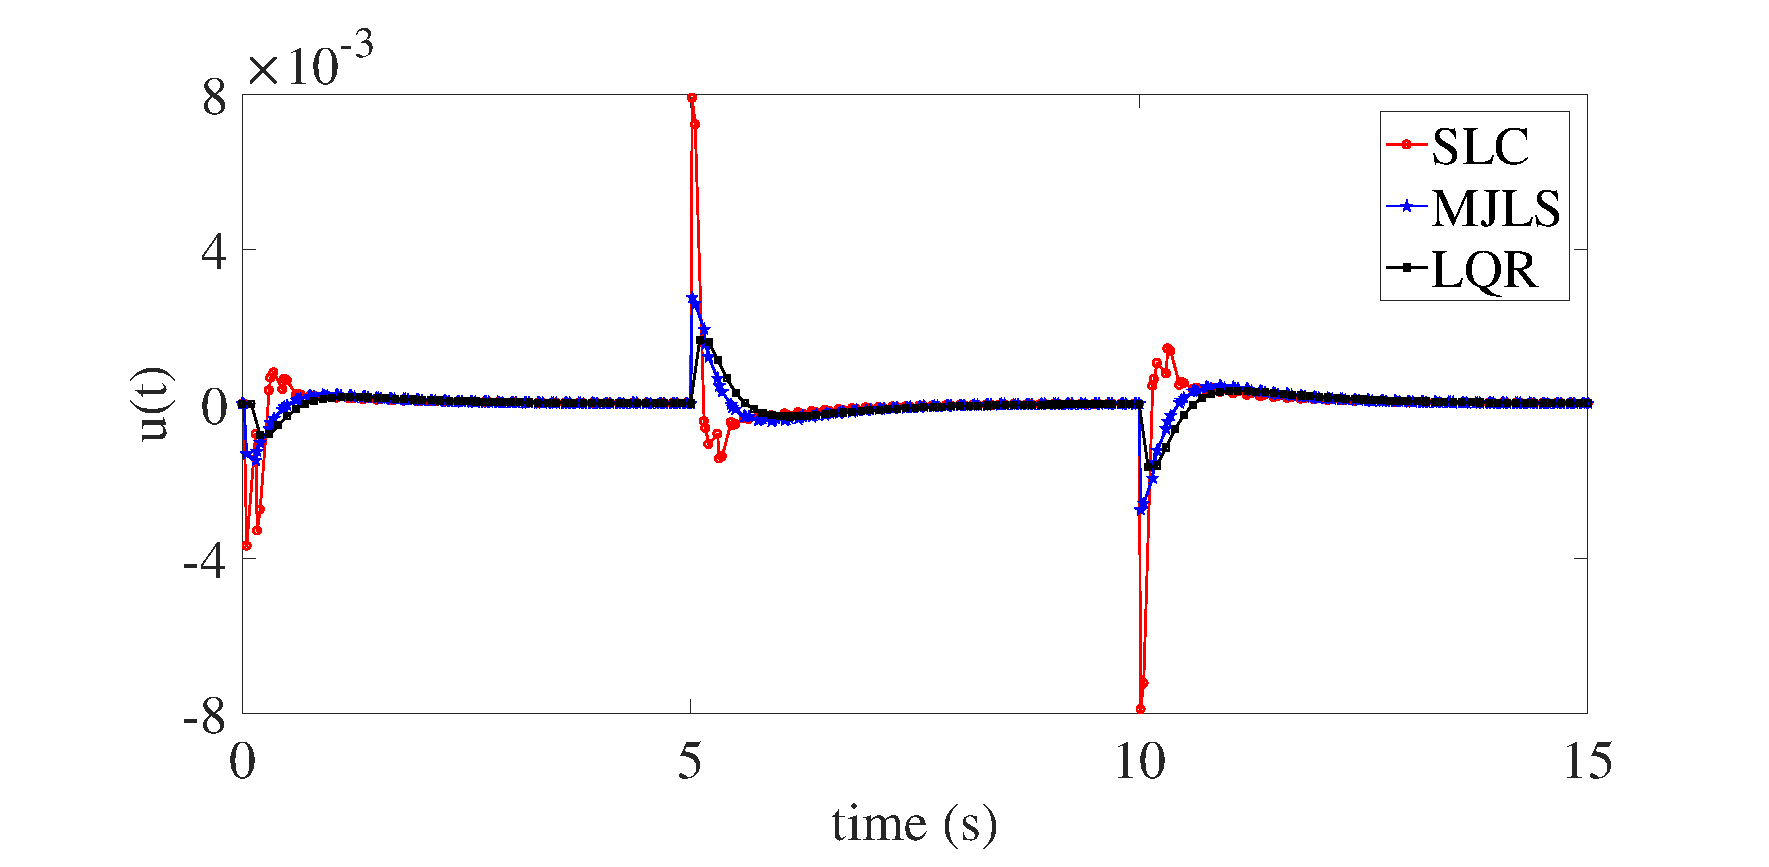
\includegraphics[width=\textwidth]{images/res_u_R1.eps}
       \caption{Input $u[k]$ when input weight $d_u=1$.}
    \end{subfigure}
    ~ 
    \begin{subfigure}[t]{0.5\textwidth}
        \centering
        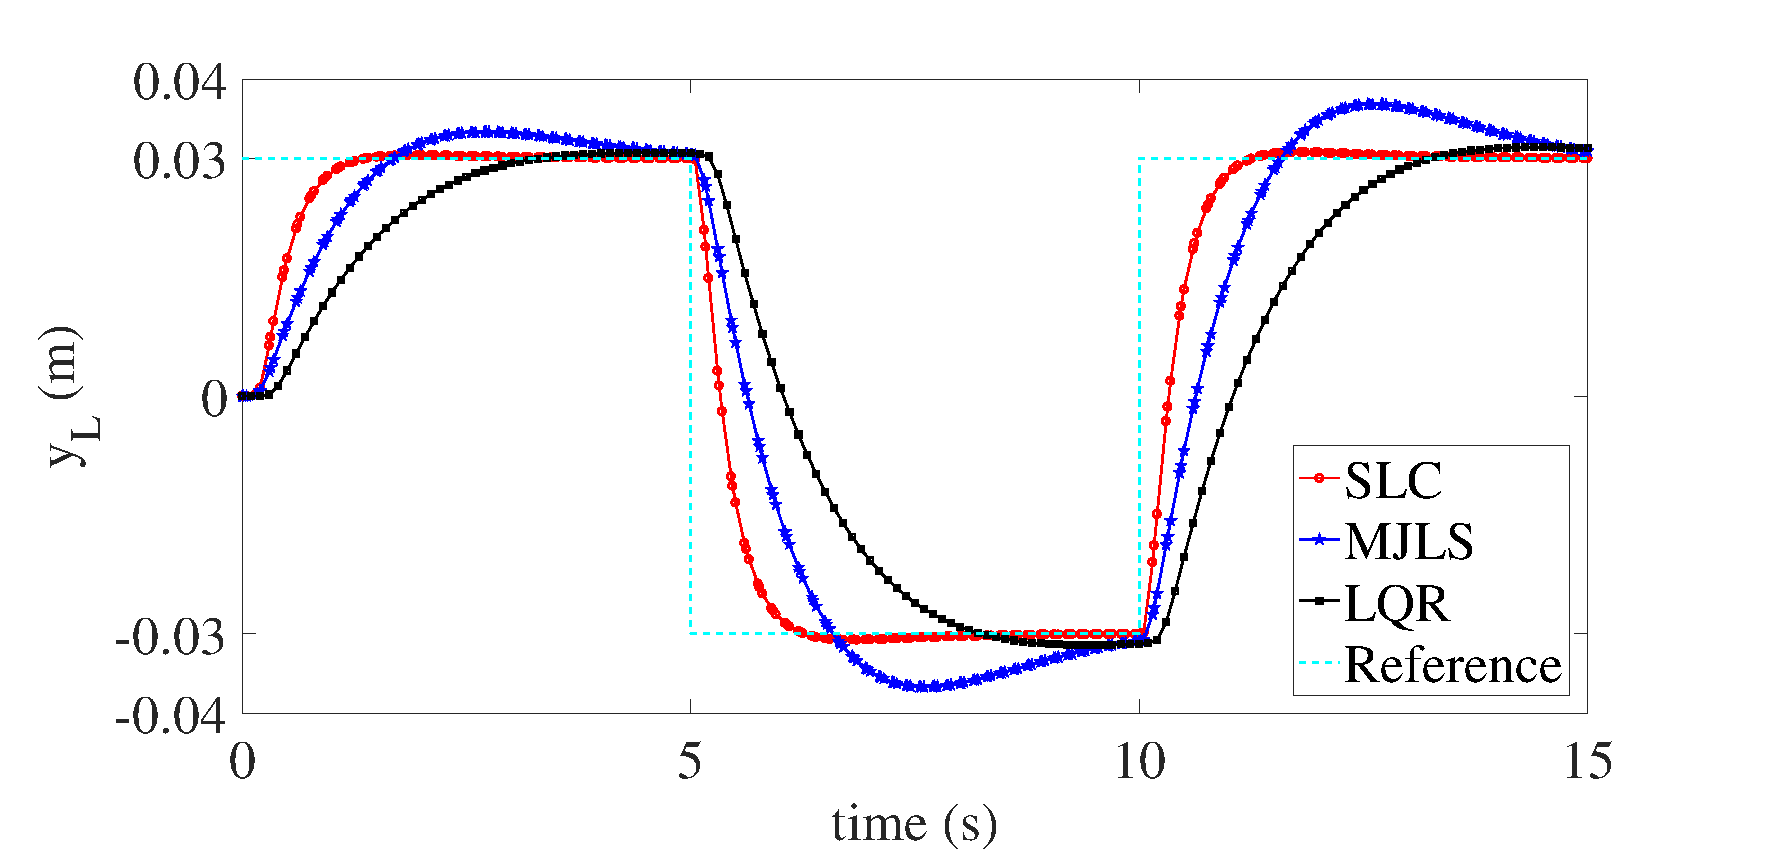
\includegraphics[width=\textwidth]{images/res_yL_R10.eps}
        \caption{Output $y_L$ when input weight $d_u=10$.}
    \end{subfigure}%
    ~
    \begin{subfigure}[t]{0.5\textwidth}
        \centering
       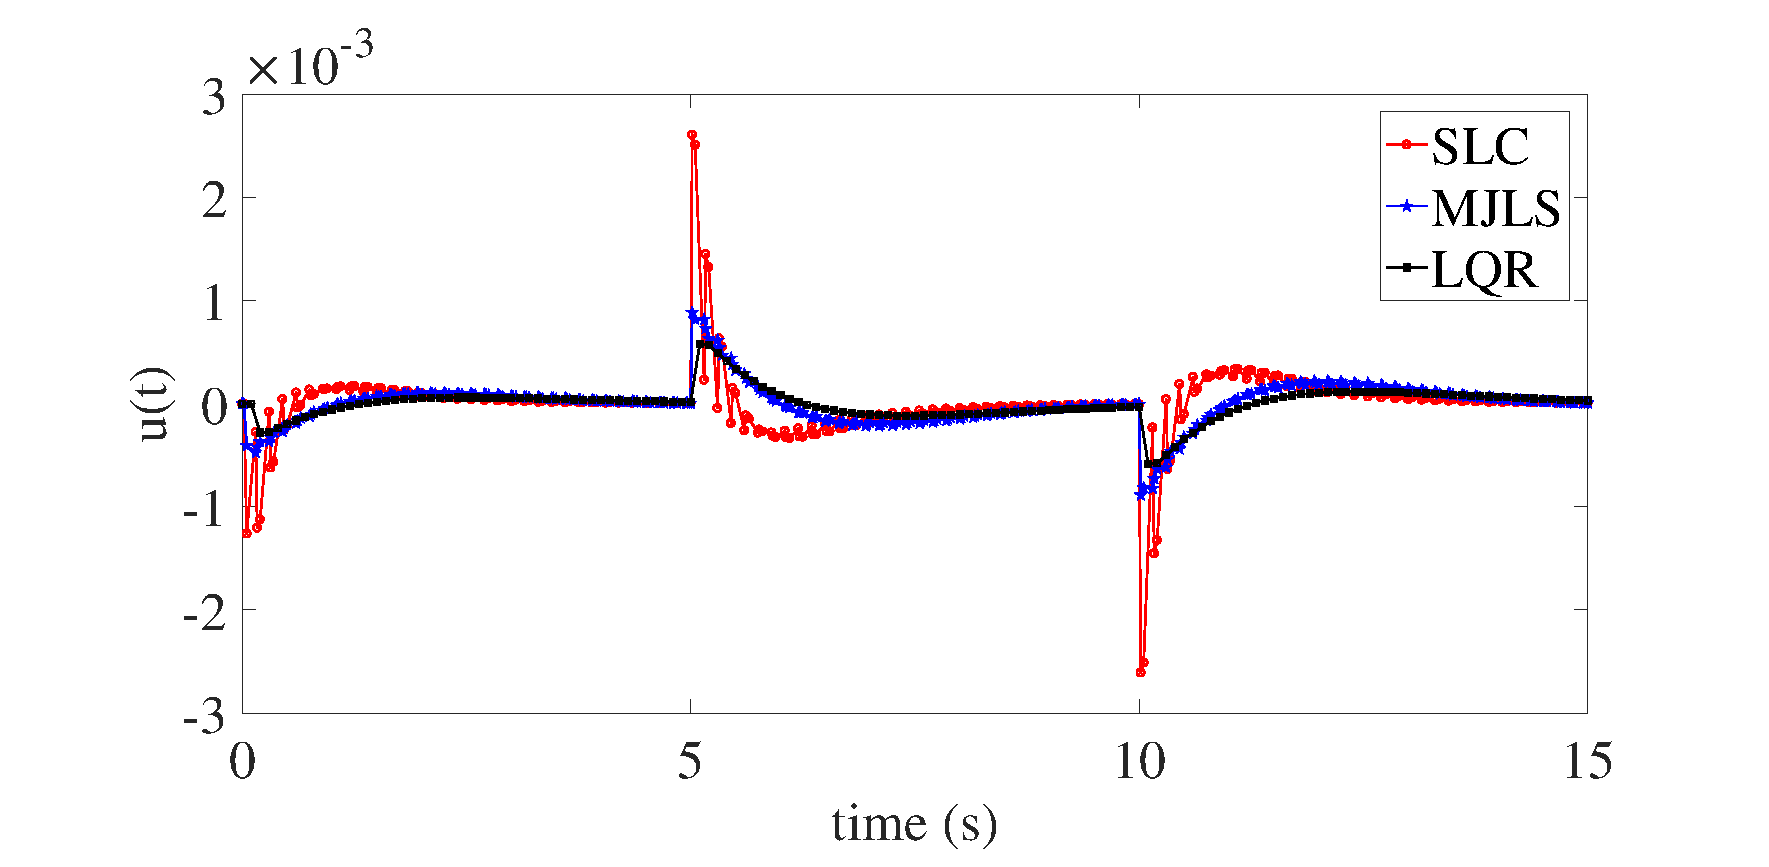
\includegraphics[width=\textwidth]{images/res_u_R10.eps}
       \caption{Input $u[k]$ when input weight $d_u=10$.}
    \end{subfigure}
    \caption{Comparison between controller synthesis method based on \gls{mjls} formulation (Section~\ref{sec:ch3_MJLS}), \gls{lqr} design (Section~\ref{sec:ch3_LQR}), and \gls{slc} system design (Section~\ref{sec:ch3_SPADe}). }
    \label{fig:ch3_results}
   \vspace{-2em}
\end{figure*}
% }
The above \gls{qoc} metrics' empirical cost for each control technique is evaluated over multiple runs of the simulation. Each simulation run generates different workload scenario sequences that satisfy the modelled \gls{dtmc}. These scenario sequences determine the switching sequence for both the \gls{slc} and \gls{mjls} control designs.


\subsection{Exploration and observations}
\label{sec:ch3_observations}
In order to provide design guidelines, we consider and vary the following different parameters: number of scenarios - we consider 3, 4 and 6 system scenarios; camera frame rates - 30 and 60 fps; input and state weights used for tuning the controllers; given platform allocation - 1, 2, 3, 4, 5, and 6 processors; and available system knowledge. We then evaluate the empirical cost of the \gls{qoc} metrics for each control technique over multiple runs of the simulation. The effects of varying these parameters are explained as follows:
\begin{enumerate}
    \item The number of states in the \gls{dtmc} model, the corresponding transition probability matrix and the number of control configurations change proportionally with the number of scenarios we consider. Only the \gls{slc} and \gls{mjls} system are affected by this parameter as the \gls{lqr} approach always (and only) considers the worst-case workload scenario;
    \item Changing the camera frame rate affects the total number of feasible scenarios we can have. As the maximum number of scenarios we can have, intuitively, is equal to $\lceil \frac{\tau_{wc}}{\fh}\rceil$, where $\tau_{wc}$ is the sensor-to-actuator delay for the worst-case workload (for a given platform allocation) and $\fh=\frac{1}{\text{camera fps}}$; 
    \item The input and state weights directly affect the control performance. E.g. for the simulation instance considered before, if we set the input weight $d_u=10$, we obtain the plots shown in Fig.~\ref{fig:ch3_results}~(c) and Fig.~\ref{fig:ch3_results}~(d). What we observe is a similar overall trend for the considered control paradigms. However, we see poorer \gls{qoc} metrics for \gls{mse} and \gls{st} and better \gls{qoc} metrics for \gls{psd} and \gls{mce}, when compared to $d_u=1$ and all other parameters remaining the same;
    \item The given platform allocation directly affects the timing parameters for a scenario $\workloadScenario$, i.e., $(h_i,\tau_i)$. A higher number of available processors mean that we could execute more tasks in parallel and reduce the  $(h_i,\tau_i)$ (even) for the worst-case workload scenario. This means that we could possibly reduce the total number of scenarios as well;
    \item System knowledge is an important parameter that determines which control design techniques can be used. An optimal control design using \gls{lqr} only requires the worst-case (workload) timing information. However,  designing an \gls{slc} system requires information regarding frequently occurring workloads as well and for the \gls{mjls} synthesis approach, we need both the frequently occurring workloads and their transition probabilities.
\end{enumerate}

\begin{table*}[t]
	\normalsize
	\begin{center}
\caption{Guidelines for choosing the control design techniques: MJLS (Section~\ref{sec:ch3_MJLS}), \gls{lqr} (Section~\ref{sec:ch3_LQR}), \gls{slc} (Section~\ref{sec:ch3_SPADe}).}
\label{Table:Results}
\scriptsize
\begin{tabular}{|c|c|c|c|c|c|}
\hline
\multirow{3}{*}{Available system knowledge}                                                                            & \multicolumn{5}{c|}{\gls{qoc} metrics}                                                                                                                                                                                                                                                                         \\ \cline{2-6} 
                                                                                                                       & \multicolumn{2}{c|}{Performance}                                                                        & \multicolumn{2}{c|}{Control energy}                                                                             & \multirow{2}{*}{\begin{tabular}[c]{@{}c@{}}Performance\\ and Energy\end{tabular}} \\ \cline{2-5}
                                                                                                                       & \gls{mse}                                                & \gls{st}                                                 & \gls{mce}                                                & \gls{psd}                                                &                                                                                      \\ \hline
Only worst-case workload information                                                                                   & \gls{lqr}                                                & \gls{lqr}                                                & \gls{lqr}                                                & \gls{lqr}                                                & \gls{lqr}                                                                                  \\ \hline
Frequently occurring workloads as a PERT                                                                               & \gls{slc}                                                & \gls{slc}                                                & \gls{lqr}                                                & \gls{lqr}                                                & \gls{slc}/ \gls{lqr}                                                                             \\ \hline
\begin{tabular}[c]{@{}c@{}}Frequently occurring workloads and their \\ transition probabilities as a \gls{dtmc}\end{tabular} & \begin{tabular}[c]{@{}c@{}}\gls{slc}/\\ MJLS\end{tabular} & \begin{tabular}[c]{@{}c@{}}\gls{slc}/\\ MJLS\end{tabular} & \begin{tabular}[c]{@{}c@{}}MJLS/\\ \gls{lqr}\end{tabular} & \begin{tabular}[c]{@{}c@{}}MJLS/\\ \gls{lqr}\end{tabular} & MJLS                                                                                  \\ \hline
\end{tabular}
\end{center}
%\horizontalEqSep
\vspace{-2em}
\end{table*}
\vspace{-0.5em}
\subsection{Design guidelines}
The design guidelines we have inferred from observing our simulations for choosing the control design techniques for different \gls{qoc} metrics and available system knowledge are listed in Table.~\ref{Table:Results}. The cases we see in the table are explained below.
\begin{itemize}
    \item \emph{Only worst-case workload information is known:}
    This situation is quite common for a control designer. Worst-case response time or delay of the algorithms can be analysed (where often times are pessimistic) through profiling and/or analytical methods~\cite{saidi2018future}. The control designer is then given only the worst-case timing information and is asked to design a controller with a \gls{qoc} requirement. In this case, the \gls{slc} and \gls{mjls} approach are not applicable and only the optimal \gls{lqr} design approach can be used. 
    
    \item \emph{PERT distribution is known:} Here, like we did in Chapters \ref{chap:parallelisation} and \ref{chap:pipelined_parallelism},  we assume that the information with respect to frequently occurring workloads is known and are characterised analytically as a PERT distribution~\cite{adyanthaya2014robustness}. In this case, \gls{slc} wins for performance-oriented metrics - \gls{mse} and \gls{st}, and \gls{lqr} wins for control effort or energy-oriented metrics - \gls{psd} and \gls{mce}. For jointly optimising performance and energy, there is no clear winner as it depends mainly on which of the two metrics is more important. If performance is important, \gls{slc} is preferred and if energy is important, \gls{lqr} should be chosen.
    The \gls{mjls} approach is not applicable as more information is needed.
    
    \item \emph{\gls{dtmc} model is known:} Information regarding frequently occurring workloads and their transition probabilities are needed for modelling a \gls{dtmc}. These can be estimated from observed workload-variations data~\cite{welton2005estimation}. Intuitively, this means that we can predict the possible (workload) scenario switching sequences for the control design. However, for the above two cases the switching sequence is assumed to be arbitrary and not known.  In this case, for performance metrics, \gls{mjls} wins when the input weight $d_u$ is very small (since \gls{slc} tends to oscillate before settling). However, for a large value of $d_u$, there is no clear winner between \gls{slc} and \gls{mjls} and it depends on the application and chosen parameters. Please note, however, that a challenge of \gls{slc} is to prove the stability of the designed system. \gls{mjls} is a synthesis method and the design, if any, is stable by construction.\\
          If we consider control effort or energy metrics, \gls{lqr} wins when the input weight $d_u$ is small and there is no clear winner between \gls{lqr} and \gls{mjls} for a large input weight $d_u$ as the results are similar and depend on the application and chosen parameters. \gls{mjls} is the clear winner if we consider a joint optimisation for performance and energy \gls{qoc} metrics.
\end{itemize}
%%%%%%%%%%%%%%%%%%%%%%%%%%%%%%%%%%%%%%%%%%%%%%%%%
%%%%%%Conclusion%%%%%%%%%%%%%%%%%%%%%%%%%%%%%%%%%
%%%%%%%%%%%%%%%%%%%%%%%%%%%%%%%%%%%%%%%%%%%%%%%%%
\section{Conclusions}~\label{sec:ch3_Conclusion}
We presented a \gls{mjls} formulation for controller synthesis for image-based control systems considering workload variations and platform implementation constraints.
Within the scope of \gls{spade}, we further compare this method with two relevant control paradigms: \gls{lqr} and switched linear control system design. 
We also provide design guidelines on the control technique to use for given constraints on the system knowledge, the \gls{qoc}, and the implementation.

The synthesis method assumes that the workload variations can be characterised as a \gls{dtmc}. A \gls{dtmc} is sensitive to the data used for its modelling. As a future work, sensitivity analysis of the \gls{dtmc} towards the \gls{qoc} needs to be evaluated. 
Further, the current design guidelines are provided based on multiple empirical simulation runs of the controller for varying workloads, number of scenarios, camera frame rate and given platform allocation. A formal mathematical analysis would strengthen our design guidelines. The challenge for a formal analysis of the control design is that we do not know the exact sequence of occurrence of the workload variations apriori.